\documentclass[11pt,a4paper]{article}
\usepackage[T1]{fontenc}\usepackage[utf8]{inputenc}
\usepackage[margin=18mm]{geometry}
\usepackage{amsmath,booktabs,longtable,graphicx,hyperref}
\title{CSA sensitivity to bias-voltage precision}
\author{NAUSICA calculation record}\date{\today}
\begin{document}\maketitle
The long decimal strings specify the numerical operating point used in the
simulation. Rounding the paper circuit's M4 and M3 gate voltages to
0.5568 and 0.5385 V preserves its gain, noise and near-linear response.
The same is true for the retuned v2 circuit with its M4 gate rounded to
0.6514 V. The exact output baseline of 0.879 V is a convenient reference
for comparing circuits; the sensitivity results establish a useful range
around that operating point.

\section*{Calculation}
The paper circuit and the retuned v2 circuit use their previously recorded
transistor dimensions. Temperature is $20\,^{\circ}$C, external input
capacitance 1.25 pF, feedback capacitance 3 fF and supply 1.8 V. One gate
voltage is varied at a time. Rounded settings change both tuned voltages
together in the paper circuit; v2 retains its M3 gate at 0.6 V.

The input is the saved mean uniform-arrival current for a 20 ms frame.
It comes from the central square 0.5 mm pad benchmark in an infinite
grounded plane, with homogeneous gas and weighting potential zero at
infinity. Ions approach through the final 5 mm at 3 m/s. Finite-path charge
$e\Delta\phi_w$ is retained without renormalization or a collection impulse.
The readout averages over centred 300 $\mu$s windows. Each bias point has
its own fitted tail constant and calibrated gain. Noise is the quiescent
output spectrum over 0.1 Hz--1 MHz after the same averaging and frame
difference. These choices match the previous circuit comparison.

Gain is obtained from the 100-ion signal. A 1000-ion transient tests its
amplitude dependence. The final table column is the relative change of
gain per ion between these two signals. This definition makes rounding
errors in calibration visible alongside the input-equivalent noise.

\section*{Rounded voltages}
\begin{center}\small\begin{tabular}{lrrrrrr}\toprule
Circuit & M3 gate (V) & M4 gate (V) & Baseline (V) & $g$ ($\mu$V/ion) & ENC ($e$) & Gain change (\%)\\\midrule
Paper & 0.538477479 & 0.556803417 & 0.879 & 27.12 & 112.72 & -0.11 \\
Paper & 0.538 & 0.557 & 1.445 & 22.51 & 110.61 & 2.74 \\
Paper & 0.5385 & 0.5568 & 0.851 & 27.04 & 112.79 & -0.11 \\
Paper & 0.53848 & 0.55680 & 0.877 & 27.11 & 112.72 & -0.11 \\
v2 retuned & 0.600000000 & 0.651398349 & 0.879 & 29.09 & 179.71 & -0.11 \\
v2 retuned & 0.600 & 0.651 & 1.003 & 29.25 & 179.91 & -0.09 \\
v2 retuned & 0.6000 & 0.6514 & 0.878 & 29.09 & 179.71 & -0.11 \\
\bottomrule\end{tabular}\end{center}

The four-decimal paper settings change ENC by 0.06\% and retain
a gain change of -0.11\% between 100 and 1000 ions. Three-decimal
rounding shifts the baseline to 1.445 V and introduces a
2.74\% gain change over the same charge range. The intrinsic ENC
remains similar, but the signal calibration becomes more amplitude-dependent.

\section*{Bias ranges}
Figure~\ref{fig:scan} shows the full scan. The following tested ranges
retain ENC within 5\% of nominal, gain within 10\% of nominal, and less
than 1\% gain change between 100 and 1000 ions:
\begin{itemize}
\item Paper M4 gate: offsets from -1 to 1 mV.
\item Paper M3 gate: offsets from -0.1 to 0.1 mV.
\item Retuned v2 M4 gate: offsets from -1 to 1 mV.
\end{itemize}
The paper M3 gate is more sensitive: offsets of $\pm0.5$ mV produce
several-percent changes in gain between 100 and 1000 ions. Across the wider
scan, the output noise can fall together with the signal gain, leaving ENC
nearly unchanged. Therefore ENC alone does not define a useful bias range.
Sufficient signal voltage and a stable charge calibration also matter for
the digitisation chain.

\begin{figure}[htbp]\centering
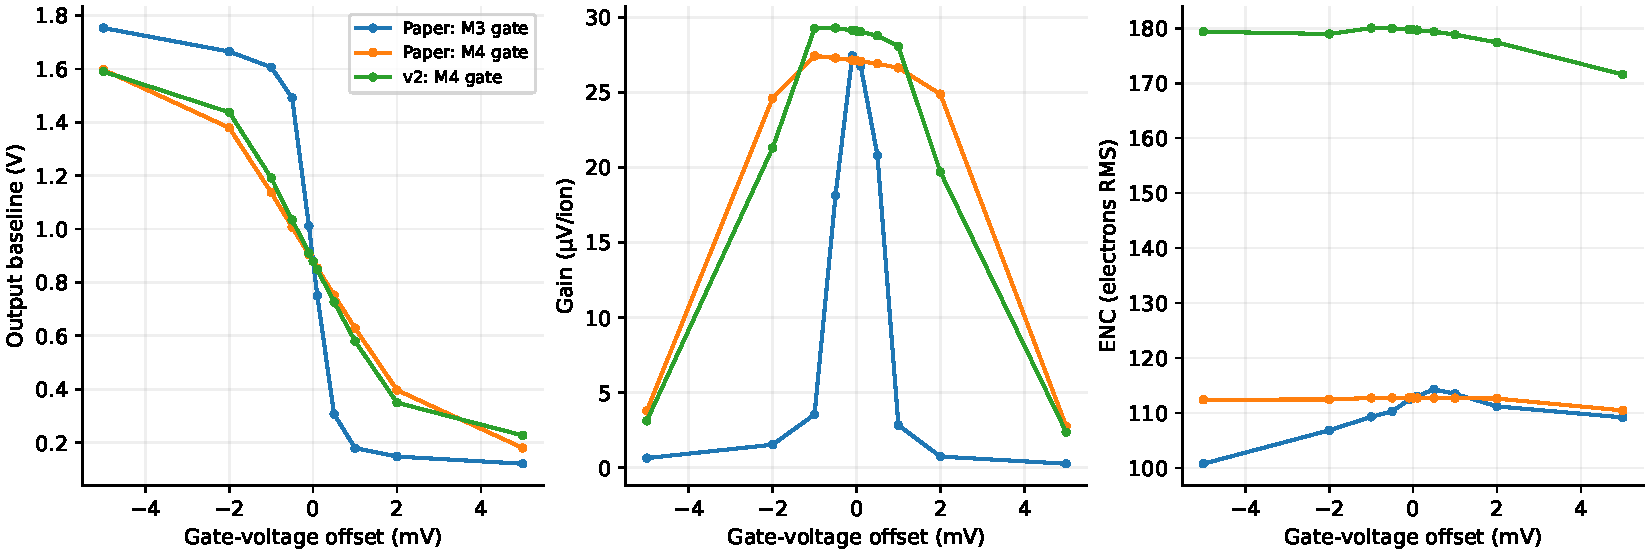
\includegraphics[width=\linewidth]{bias_sweep.pdf}
\caption{One gate varied at a time, with the other biases fixed.}
\label{fig:scan}\end{figure}

The four-decimal values are adequate for reporting the present operating
point and reproducing its performance. A practical circuit can trim or
calibrate its bias to a suitable operating region. This scan uses the supplied
model at one temperature; process and temperature scans would determine
the adjustment range needed in hardware.

\section*{Checks and reproduction}
The rounded settings and representative offset points use paired maximum
steps of 5 and 2.5 $\mu$s with tightened solver tolerances, noise spectra
at 200 and 400 points per decade, and quadrature orders 8 and 16.
Input-charge conservation is checked for every point. The stored analyses
include the output extrema for 1000 ions and the input-node voltage shift.

Configuration is \texttt{config/bias\_sensitivity.toml}; Julia reduction is
\texttt{src/ion\_signal/bias\_sensitivity.jl}. Reproduction commands and the
list of refined points are in \texttt{results/ltspice/bias\_sensitivity/README.md}.
Python generates this report from \texttt{analysis.h5}.

\section*{Complete scan}
Indices 1--11 correspond to gate offsets
$-5,-2,-1,-0.5,-0.1,0,0.1,0.5,1,2,5$ mV.
\small
\begin{longtable}{lrrrrrr}\toprule
Case & M3 (V) & M4 (V) & Baseline (V) & $g$ ($\mu$V/ion) & ENC ($e$) & Gain change (\%)\\\midrule\endhead
paper\_m3\_1 & 0.5334775 & 0.5568034 & 1.753 & 0.64 & 100.74 & 0.38 \\
paper\_m3\_10 & 0.5404775 & 0.5568034 & 0.148 & 0.75 & 111.18 & -1.40 \\
paper\_m3\_11 & 0.5434775 & 0.5568034 & 0.121 & 0.27 & 109.18 & -0.38 \\
paper\_m3\_2 & 0.5364775 & 0.5568034 & 1.665 & 1.54 & 106.82 & 0.83 \\
paper\_m3\_3 & 0.5374775 & 0.5568034 & 1.606 & 3.55 & 109.28 & 2.92 \\
paper\_m3\_4 & 0.5379775 & 0.5568034 & 1.491 & 18.13 & 110.26 & 5.39 \\
paper\_m3\_5 & 0.5383775 & 0.5568034 & 1.011 & 27.44 & 112.39 & -0.10 \\
paper\_m3\_6 & 0.5384775 & 0.5568034 & 0.879 & 27.12 & 112.72 & -0.11 \\
paper\_m3\_7 & 0.5385775 & 0.5568034 & 0.750 & 26.76 & 113.03 & -0.13 \\
paper\_m3\_8 & 0.5389775 & 0.5568034 & 0.307 & 20.80 & 114.28 & -3.47 \\
paper\_m3\_9 & 0.5394775 & 0.5568034 & 0.179 & 2.84 & 113.46 & -4.71 \\
paper\_m4\_1 & 0.5384775 & 0.5518034 & 1.597 & 3.79 & 112.39 & 3.26 \\
paper\_m4\_10 & 0.5384775 & 0.5588034 & 0.397 & 24.89 & 112.60 & -1.04 \\
paper\_m4\_11 & 0.5384775 & 0.5618034 & 0.180 & 2.76 & 110.45 & -4.71 \\
paper\_m4\_2 & 0.5384775 & 0.5548034 & 1.379 & 24.61 & 112.45 & 1.01 \\
paper\_m4\_3 & 0.5384775 & 0.5558034 & 1.137 & 27.43 & 112.71 & -0.08 \\
paper\_m4\_4 & 0.5384775 & 0.5563034 & 1.007 & 27.29 & 112.72 & -0.10 \\
paper\_m4\_5 & 0.5384775 & 0.5567034 & 0.904 & 27.15 & 112.72 & -0.11 \\
paper\_m4\_6 & 0.5384775 & 0.5568034 & 0.879 & 27.12 & 112.72 & -0.11 \\
paper\_m4\_7 & 0.5384775 & 0.5569034 & 0.854 & 27.08 & 112.71 & -0.11 \\
paper\_m4\_8 & 0.5384775 & 0.5573034 & 0.753 & 26.91 & 112.70 & -0.13 \\
paper\_m4\_9 & 0.5384775 & 0.5578034 & 0.629 & 26.63 & 112.68 & -0.18 \\
paper\_rounded\_3 & 0.5380000 & 0.5570000 & 1.445 & 22.51 & 110.61 & 2.74 \\
paper\_rounded\_4 & 0.5385000 & 0.5568000 & 0.851 & 27.04 & 112.79 & -0.11 \\
paper\_rounded\_5 & 0.5384800 & 0.5568000 & 0.877 & 27.11 & 112.72 & -0.11 \\
v2\_m4\_1 & 0.6000000 & 0.6463983 & 1.590 & 3.12 & 179.37 & 2.80 \\
v2\_m4\_10 & 0.6000000 & 0.6533983 & 0.350 & 19.70 & 177.41 & -5.20 \\
v2\_m4\_11 & 0.6000000 & 0.6563983 & 0.227 & 2.37 & 171.58 & -3.28 \\
v2\_m4\_2 & 0.6000000 & 0.6493983 & 1.437 & 21.30 & 178.95 & 3.43 \\
v2\_m4\_3 & 0.6000000 & 0.6503983 & 1.192 & 29.27 & 180.03 & 0.17 \\
v2\_m4\_4 & 0.6000000 & 0.6508983 & 1.034 & 29.29 & 179.95 & -0.08 \\
v2\_m4\_5 & 0.6000000 & 0.6512983 & 0.910 & 29.14 & 179.77 & -0.10 \\
v2\_m4\_6 & 0.6000000 & 0.6513983 & 0.879 & 29.09 & 179.71 & -0.11 \\
v2\_m4\_7 & 0.6000000 & 0.6514983 & 0.848 & 29.04 & 179.65 & -0.11 \\
v2\_m4\_8 & 0.6000000 & 0.6518983 & 0.727 & 28.77 & 179.36 & -0.17 \\
v2\_m4\_9 & 0.6000000 & 0.6523983 & 0.580 & 28.06 & 178.83 & -0.43 \\
v2\_rounded\_3 & 0.6000000 & 0.6510000 & 1.003 & 29.25 & 179.91 & -0.09 \\
v2\_rounded\_4 & 0.6000000 & 0.6514000 & 0.878 & 29.09 & 179.71 & -0.11 \\
v2\_rounded\_5 & 0.6000000 & 0.6514000 & 0.878 & 29.09 & 179.71 & -0.11 \\
\bottomrule\end{longtable}
\end{document}
